\section{D.C. Circuits}
\textbf{Direct current} (d.c.): current flowing only in \emph{one direction}

\subsection{Circuit symbols and diagrams}
Circuit symbols:

\begin{figure}[H]
    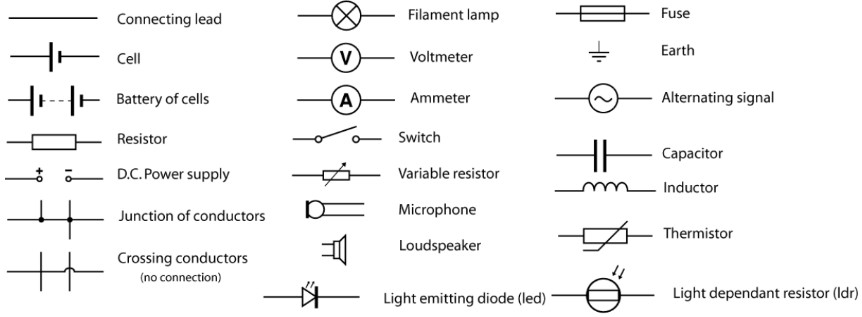
\includegraphics[width=16cm]{images/circuit_symbols.jpg}
\end{figure}

\subsection{Series and parallel arrangements}
\subsubsection{Current}
Current divides up where a circuit splits into multiple branches. 
\begin{defn}{Kirchhoff’s Current Law}{}
Algebraic sum of the currents at a junction of a circuit is zero.
\begin{equation}
\sum_{\text{junction}}I_i=0
\end{equation}
Currents entering the junction are given a positive $(+)$ sign, currents leaving the junction are given a negative $(-)$ sign.
\end{defn}

This means sum of currents entering a junction = sum of currents leaving the junction
\[ \sum I_\text{in} = \sum I_\text{out} \]

\begin{proof}
By the Principle of Conservation of Charge, the total charge that enters a junction per unit time must be equal to the total charge that leaves the same junction per unit time.
\end{proof}

\paragraph{Series}
Currents at all points are same, equal to total current.
\[ I_1=\cdots=I_n=I \]

\paragraph{Parallel}
Total current is sum of individual currents.
\[ I = I_1+\cdots+I_n \]

\subsubsection{Voltage}
\begin{defn}{Kirchhoff’s Voltage Law}{}
Algebraic sum of all electrical potential changes around any closed loop is zero.
\begin{equation}
\sum_{\text{junction}}\Delta V_i=0
\end{equation}
\end{defn}

This means the sum of the e.m.f.s around any loop in a circuit is equal to the sum of the p.d.s around the loop.
\[ \sum \epsilon = \sum V_\text{drop} \]

\begin{proof}
By the Law of Conservation of Energy, energy supplied by the source is equal to energy dissipated by resistors.

For constant current and time,
\begin{align*}
\brac{I\sum\epsilon}t &= \brac{I^2\sum R}t \\
\sum\epsilon &= I\sum R \\
\sum\epsilon &= \sum V
\end{align*}
\end{proof}

\begin{remark}
Current always flows from higher potential to lower potential.
\end{remark}

\paragraph{Series}
e.m.f. is sum of voltages.
\[ V_1+\cdots+V_n = \epsilon \]

\paragraph{Parallel}
Voltages are same, equal to e.m.f.
\[ \epsilon = V_1=\cdots=V_n \]

\subsubsection{Resistance}
\paragraph{Series}
Effective resistance is sum of individual resistances

\begin{equation}
R_{\text{eff}} = R_1 + \cdots + R_n
\end{equation}

\begin{derivation}
Consider two resistors of resistances $R_1$ and $R_2$ connected in series. 

According to Kirchhoff’s current law, the current in each resistor is the same. The p.d. $V$ across the combination is equal to the sum of the p.d.s across the two resistors:
\[ V = V_1+V_2 \]
Since $V = IR$, $V_1 = IR_1$ and $V_2 = IR_2$, we can write:
\[ IR = IR_1+IR_2 \]
Cancelling the common factor of current $I$ gives:
\[ R = R_1+R_2 \]
For three or more resistors, the equation for total resistance $R$ becomes:
\[ R = R_1+R_2+R_3+\cdots \]
\end{derivation}

\paragraph{Parallel}
Reciprocal of effective resistance is sum of reciprocals of individual resistances

\begin{equation}
\frac{1}{R_\text{eff}} = \frac{1}{R_1} + \cdots + \frac{1}{R_n}
\end{equation}

\begin{remark}
Effective resistance of resistors in parallel is always lower than the lowest resistance in the network.
\end{remark}

\begin{derivation}
Consider two resistors of resistances $R_1$ and $R_2$ connected in parallel. The total current is divided between them. 

Using Kirchhoff's current law,
\[ I = I_1+I_2 \]
Applying Kirchhoff's voltage law to the loop that contains the two resistors,
\[ I_1R_1 - I_2R_2 = 0 \]
(because there is no source of e.m.f. in the loop)

This suggests that the two resistors have the same p.d. across them. Hence we can write $I=\frac{V}{R}$, $I_1=\frac{V_1}{R_1}$ and $I_2=\frac{V_2}{R_2}$.

Substituting these into $I = I_1+I_2$ and cancelling the common factor $V$,
\[ \frac{1}{R} = \frac{1}{R_1} + \frac{1}{R_2} \]

For three or more resistors, the equation for total resistance $R$ becomes
\[ \frac{1}{R} = \frac{1}{R_1} + \frac{1}{R_2} + \frac{1}{R_3} + \cdots \]
\end{derivation}

\subsubsection{Measuring instruments}
\begin{table}[H]
\centering
\begin{tabular}{|c|c|c|c|}
\hline
\textbf{Instrument} & \textbf{Measured quantity} & \textbf{Assumption}\footnote{unless stated otherwise} & \textbf{Connection} \\
\hline
\textbf{ammeter} & current (in one direction) & zero (internal) resistance & in series \\
\textbf{galvanometer} & current (in both directions) & zero (internal) resistance & in series \\
\textbf{voltmeter} & potential difference & infinite resistance & in parallel \\
\hline
\end{tabular}
\end{table}

\subsection{Potential divider}
\begin{defn}{Potential divider rule}{}
If a voltage exists across several resistors connected in series, then the voltage across each resistor is proportional to the total resistance.
\begin{equation}
V_1 = \frac{R_1}{R_T}V
\end{equation}
\end{defn}

\begin{derivation}
Consider two resistors $R_1$ and $R_2$ are connected in \emph{series}. The \emph{same} current flows through both resistors.

Hence p.d. across $R_1$ is given by
\[ V_1 = IR_1 = \brac{\frac{E}{R_1+R_2}}R_1 = \brac{\frac{R_1}{R_1+R_2}}E \]
or
\[ \frac{V_1}{E} = \frac{R_1}{R_T} \]
This means that the two resistors divide the total p.d. into fractions according to their resistance.
\end{derivation}

Using the potential-divider principle for a continuous resistor (e.g. a resistance wire) which has constant resistance per unit length, the voltage drop across a section of the wire $AB$ is proportional to the length of $AB$ as a fraction to the wire's total length.
\[ V_{AB} = \frac{\ell_{AB}}{\ell_T} \times V \]

\begin{tcolorbox}
Consider a wire of non-uniform resistance per unit length, who resistance is described by the function $R(x)$. Integrating over the length of the wire $L$ gives the total resistance of the wire:
\[ R = \int_0^L R(x) \dd{x} \]
where the length $x$ is measured from one fixed end of the wire.
\end{tcolorbox}

\subsubsection{Potentiometer}
A \vocab{potentiometer} is a device used for comparing potential differences \emph{without drawing a current}\footnote{This is in contrast to a voltmeter. A non--ideal voltmeter draws some current from the circuit as it does not have infinitely high resistance.} from the circuit involved. It is used to measure the unknown e.m.f. of a source $E_1$, using another source of known e.m.f. $E_0$.

\begin{figure}[H]
    \centering
    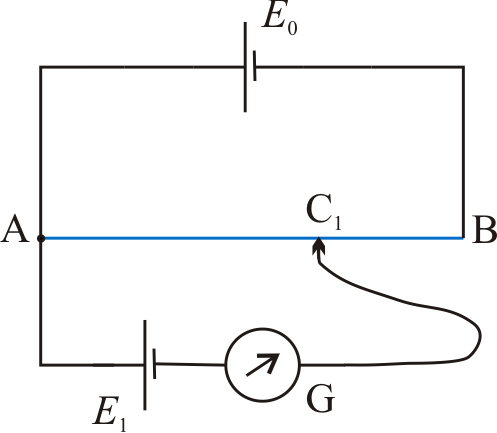
\includegraphics[width=6cm]{images/potentiometer.png}
\end{figure}

\begin{proposition}
Along the slide wire, $V \propto \ell$.
\end{proposition}
\begin{proof}
p.d. across $AB$ is
\[ V_{AB} = IR_{AB} = I\brac{\frac{\rho\ell_{AB}}{A}} \]
Similarly, p.d. across $AY$ is
\[ V_{AC} = IR_{AC} = I\brac{\frac{\rho\ell_{AC}}{A}} \]
Hence it is evident that 
\[ \frac{V_{AC}}{V_{AB}} = \frac{\ell_{AC}}{\ell_{AB}} \implies \boxed{V \propto \ell} \]
\end{proof}

\begin{remark}
Recall that there needs to be a potential difference for current to flow.
\end{remark}

\textbf{Objective:} Locate the \textbf{balance point} to determine \textbf{balance length}.
\begin{itemize}
\item At the balance point, No current flows through galvanometer. Galvanometer registers zero reading.
\item This means no potential difference between point $A$ and $+$ve terminal of $E_1$, and between point $C$ and $-$ve terminal of $E_1$. Hence p.d. between $A$ and $C$ is equal to p.d. across $E_1$, thus $E_1=V_{AC}$.
\item Since p.d. is proportional to length across slide wire, we have 
\[ E_1 = V_{AC} = \frac{\ell_{AC}}{\ell_{AB}}V_{AB} \]
\end{itemize}

\subsubsection{Wheatstone bridge}
The Wheatstone bridge is a way to measure the resistance of unknown resistors placed in the position of $R_4$, where the resistance of variable resistor $R_3$ is adjustable.

\begin{figure}[H]
    \centering
    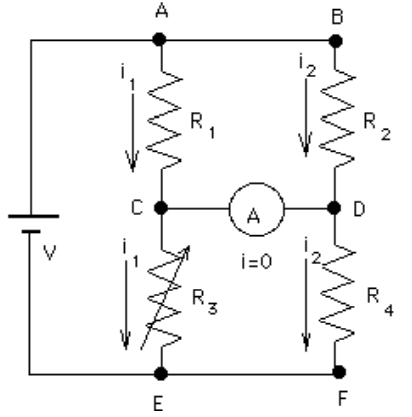
\includegraphics[width=8cm]{images/wheatstone.png}
\end{figure}

Since no current flows in the ammeter, no potential difference between points $C$ and $D$. Hence $V_C=V_D$.

Since no current flows through the ammeter, $I_1=I_3$ and $I_2=I_4$. It also follows (from the fact that points C and D have the same potential) that the voltage drop across $R_1$ is the same as the voltage drop across resistor $R_2$. Hence
\begin{equation*}\tag{1}
I_1 R_1 = I_2 R_2
\end{equation*}

Similarly, voltage drop across $R_3$ is the same as voltage drop across $R_4$ so
\begin{equation*}\tag{2}
I_1 R_3 = I_2 R_4
\end{equation*}

Dividing (1) by (2) gives us
\begin{equation*}\tag{3}
\frac{R_1}{R_3} = \frac{R_2}{R_4}
\end{equation*}

Solving (3) for the unknown resistor $R_4$,
\[ R_4 = \frac{R_2}{R_1}R_3 \]
\pagebreak

\subsection*{Problems}
\begin{prbm}[M\"{o}bius Strip]
Two wires are each strung with 4 resistors, along with another 4 resistors that bridge pairs of resistors across both wires. The wires are then twisted together to form a M\"{o}bius strip, as shown below.

\begin{figure}[H]
    \centering
    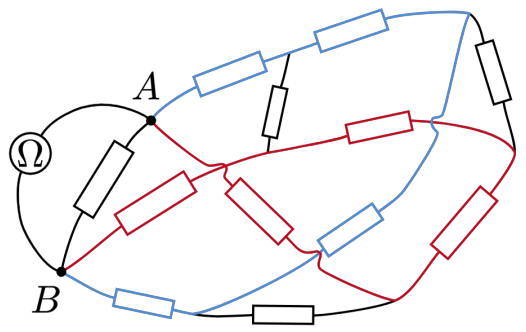
\includegraphics[width=7cm]{images/Mobius_strip.png}
\end{figure}

Every resistor has identical resistance $R = 1.0\:\Omega$. Determine the equivalent resistance $R_{eq}$ between the points $A$ and $B$ in the M\"{o}bius strip.

\textit{Leave your answer to 2 significant figures in units of $\Omega$.}
\end{prbm}

\begin{solution}
Imagine ``slicing" the M\"{o}bius strip along line AB and then opening up and untwisting the circuit. The circuit can then be redrawn in its deconstructed form:

\begin{figure}[H]
    \centering
    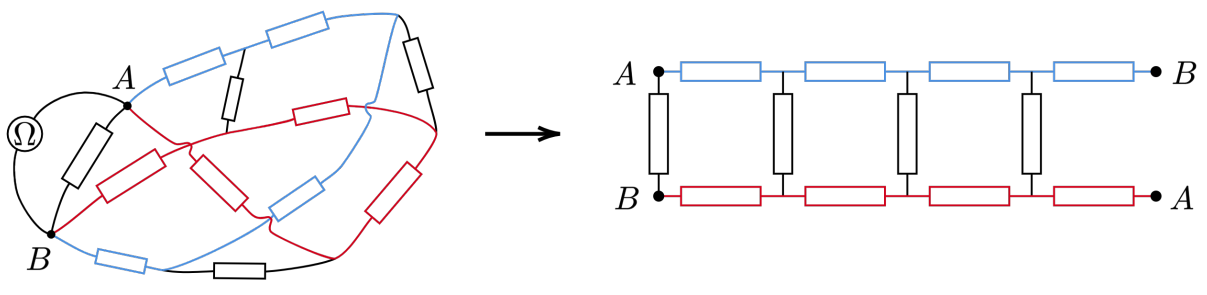
\includegraphics[width=15cm]{images/Mobius_strip_1.png}
\end{figure}

To determine the resistance $R_{eq}$ across $AB$, we can treat the 1 bridging resistor, of resistance $R$, to be in parallel with the rest of the circuit, of unknown resistance $R^\prime$.

\begin{figure}[H]
    \centering
    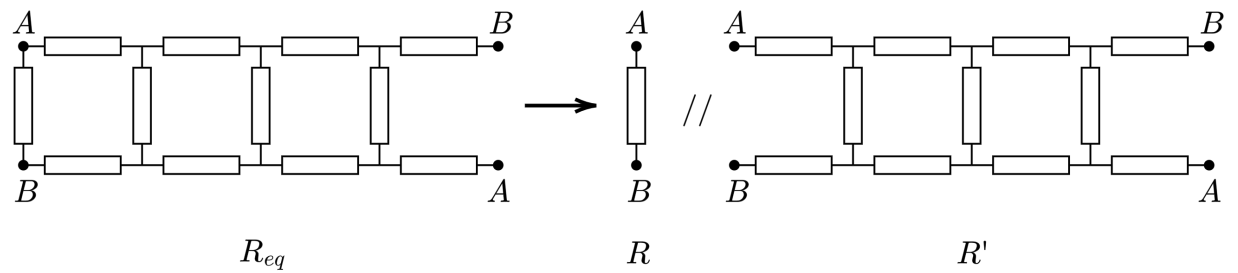
\includegraphics[width=15cm]{images/Mobius_strip_2.png}
\end{figure}

Let us now focus on finding this unknown resistance $R^\prime$. Notice that due to the symmetry of this circuit, there are 3 pairs of equipotential points as marked below (each pair takes a different colour). As such, we obtain the following equivalent circuit after combining points $A$ and $B$ on both ends:

\begin{figure}[H]
    \centering
    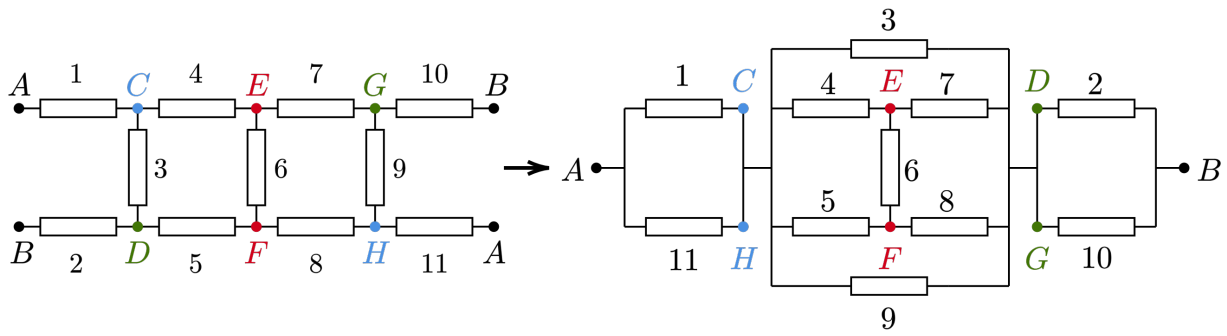
\includegraphics[width=15cm]{images/Mobius_strip_3.png}
\end{figure}

From here, we can determine the value of $R^\prime$ (noting that resistor 6 can be disregarded since its two ends are equipotential):

\[ R^\prime = \frac{1}{\frac{1}{R}+\frac{1}{R}} + \frac{1}{\frac{1}{R}+\frac{1}{2R}+\frac{1}{2R}+\frac{1}{R}} + \frac{1}{\frac{1}{R}+\frac{1}{R}} = \frac{4}{3}R \]

We can hence calculate the resistance $R_{eq}$ of the complete circuit:

\[ R_{eq} = \frac{1}{\frac{1}{R}+\frac{1}{R^\prime}} = \frac{4}{7}R \approx \boxed{0.57\:\Omega} \]
\end{solution}
\pagebreak

\begin{prbm}[Hexagonmania]
Roger is bored, so he decides to use his collection of uniform thin copper rods, each of resistance $R = 1.00\:\Omega$, to create a rigid compound shape shown below. The copper rods form seven regular hexagons. Calculate the effective resistance $R_{AB}$ between points $A$ and $B$.

\textit{Leave your answer to 3 significant figures in units of $\Omega$.}
\end{prbm}

\begin{solution}
% https://sgphysicsleague.org/archives/2023/solutions.pdf Problem 38
\end{solution}
\pagebreak